%% rsync <=> delta file algorithms

\documentclass[]{article}
\usepackage{sectsty}
\usepackage[parfill]{parskip}
\usepackage{hyperref}
\usepackage[T1]{fontenc}
\usepackage[T1]{fontenc}
%%images
\usepackage{graphicx}
%%\graphicspath{ {images/} }

\sectionfont{\fontsize{10}{10}\selectfont}

\begin{document}
%%Authors
\author{
  Kabir Chhabra\\
  \texttt{2013CS50287}
  \and
  Harman Kumar\\
  \texttt{2013CS10224}
  \and  
  Haroun Habeeb\\
  \texttt{2013CS10225}
}
\title{COP 290 Assignment 2}
\maketitle

%%\begin{center}
%%
\includegraphics[width = 10cm]{images/hello1.jpg}
%%\end{center}


%%Abstract
\begin{abstract}
This is the design document for an application called myDropBox. The application allows a user to upload files onto a server. He can access the files present on a server from any pc. \\
Every user can share a certain directory on a linux machine.
\end{abstract}

\section{Overall Design}
\begin{center}
Developed using : \textbf{QtCreator} \\
Developed for   : \textbf{Linux systems}\\
Security ensured: \textbf{openSSL}\\
Communication using: \textbf{socket programming}\\
\end{center} 

Classes :
\begin{enumerate}
\item \textbf{Server}
\begin{itemize}
\item Console based applicated
\item Uses fork() to handle multiple clients
\item Stores data in seperate directories.
\item Stores delta files for each file
\end{itemize}
\item \textbf{Client}
\begin{itemize}
\item minimalistic GUI:
\begin{enumerate}
\item LoginScreen
\item RegisterScreen
\item myDropBox (mainWindow)
\end{enumerate}
\end{itemize}

\end{enumerate}


%%
\section{\LARGE Project Structure}
%%Describe classes etc.
Our project is divided into the following primary parts - the server, the client and the algorithms involved.
Since each of the three parts is highly modular, we will have a file for each module, for example, we will have a file for authentication on the server side, another file for authentication of the client side etc. \\
We will now describe all of our subcomponents.
%%
\subsection{Server}
The server is a C++ console application running on a computer. It allows for multiple clients to connect at any given time. It achieves this by invoking the \textit{fork()} method. \\
The server also has multiple back-end modules such as ping(for testing), authentication, registration, file uploads and file downloads, file sharing, searching for files etc. \\
The list of functions is server are:
\begin{itemize}
\item \textbf{startServer():}  This initializes the server object, creates the host socket of the server. 
\item \textbf{getClient():}    This function accepts new clients and forks to create a new process which handles the new client.
\item \textbf{handleClient():} This function is a loop which handles a connection from a server. As the socket closes, the process is also freed. Using fork() is justified because that is in essence what needs to be done. Also, fork() is very commonly used, by big names such as Apache.
\item \textbf{Modules:}
Every back-end module or feature of the application is coded up in a very modular manner. We will have an authentication module, a module for registration, a few modules for the file transfer, some modules for sharing, some modules for version control, some for utility - like reading and writing to the buffer securely. Each module can be developed independtly once the modules it depends on are developed.
\end{itemize}

\subsection{Client}
The client application is a functional, graphical UI. The UI will be implemented using Qt and its various form-creating facilities. The front-end itself will be minimalistic.
The back-end of the client can be divided into a few parts:
\begin{itemize}
\item \textbf{File Handling:}
Every client needs to keep track of the versions of various files that are in the clients directory. The application makes decisions based on these parameters which are saved in a hidden file in the client's directory.
\item \textbf{Communication:}
Communicaiton between client and server happens through sockets. We have a predefined set of instructions, including an end-instruction (special token). The transfer of data is synchronized using \textit{poll()} function provided by linux.
\item \textbf{Error Handling:}
Occasionally, file conflicts and errors happen - the server handles these errors by instructing the client to do specific actions. For example, if the client tries to push a previous version, the server will need to handle the request. However, the client will be implementing these changes.
\end{itemize}
%%\subsection{Communications} The communication between client and server is done by passing "instructions" over the internet. The server accepts these instructions using a "getInstruction()" method and handles the instructions using a "handleInstructions()" method. 

\subsection{File Handling}
%%TODO : Descibe GUI :Done
The file can be read and delta files can be computed in many ways. The diff, rsync tools are simple implementations that are readily available on linux machines. They return the optimal delta file.
Another issue that is declared in various sections that directly deal with files - storage, sharing etc.
The gist of the issue is a manifesto - one in the client directory and another in the server directory.
Some of the various algorithms which we can use are :
\begin{itemize}
\item diff
\item rsync
\item librsync by dropbox
\end{itemize}

\section{\LARGE User Interface}
%%TODO : INSERT IMAGES HERE
\subsection{LoginForm}
\begin{center}
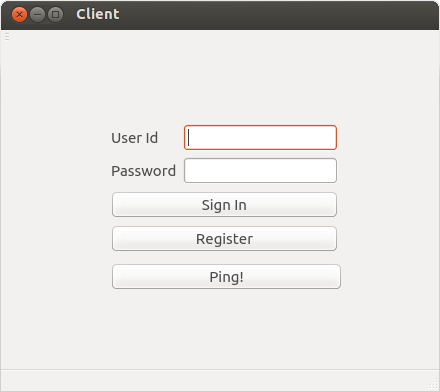
\includegraphics[scale=0.4]{images/img_login.png}
\end{center}
We will be using a very simple, rudimentary login screen. It has a field for username, a field for password, a sign-in button and a register button(to add new users). Authentication will be done entirely on the server side. 
The buttons are :
\begin{itemize}
\item UserId: To enter the username.
\item Password: To enter password.
\item Sign In: Opens up the user's Main Window if the credentials are correct. this will be where the user interacts with myDropBox.
\item Register: This opens up the register window where the user can sign up for a myDropBox account.
\end{itemize}



\subsection{RegisterForm}
\begin{center}
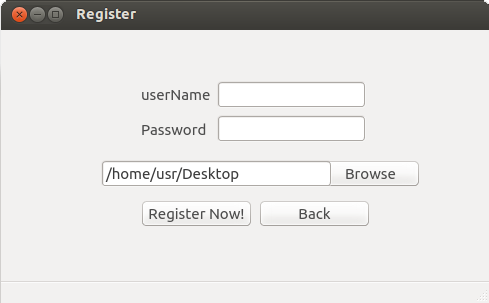
\includegraphics[scale=0.4]{images/img_register.png}
\end{center}

The register form will be a minimalistic one which asks you for a desired username and password and a working directory from which to share files. The password is confirmed in a separate field. It is ensured that the same userId doesn't already exist on the server. 
The buttons are :
\begin{itemize}
\item UserId: To enter the username.
\item Password: To enter Password.
\item Register: To sign up for an account. If the entry is accepted, the account is created and the user is redirected to the login screen.  
\end{itemize}

\subsection{MainWindow}
\begin{center}
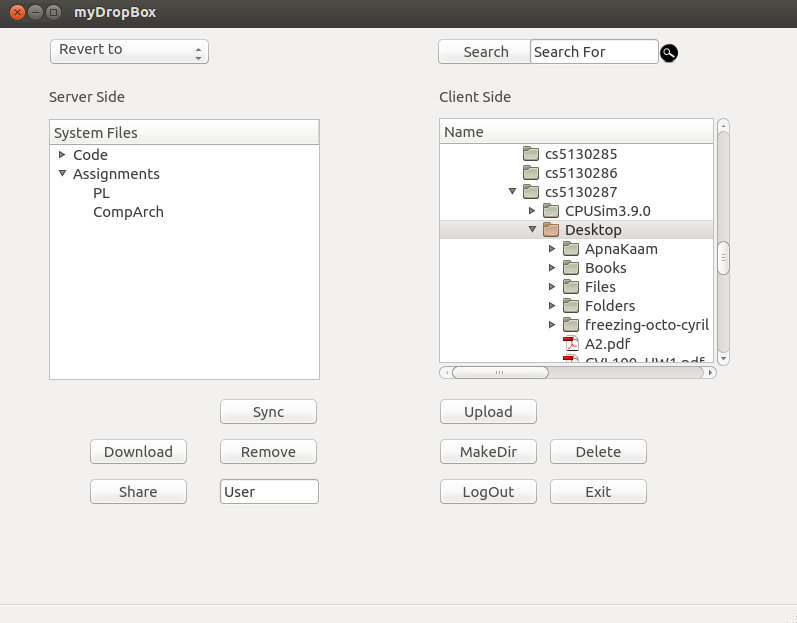
\includegraphics[scale=0.4]{images/img_mdb.png}
\end{center}
The MainWindow is the area where the user interacts with the server. Facilities are provided for uploading, downloading, syncing the repository. An interactive search feature and a share feature enables the user to share his files with other users. Deleting, moving the files between directories and logging out can be achieved at the click of a button. A file tree is used to depict the files of the user on the system, and another for the files on the server. A revert option is given to retrieve earlier versions of a particular file.
The buttons are :
\begin{itemize}

\item Upload		: To upload the selected file to the server.
\item Download		: To download the selected file to the client's system.
\item Search		: To search for files which the user has access to. 
\item Share		: To share the selected file/folder with a particular user.
\item Remove		: To remove a particular file from the server/client system.
\item MakeDir	: To make a new directory in the users system.
\item Delete		: To delete directories in the users system.
\item Move		: To move files from one directory to the other on the clients system.
\item Sync		: To sync the Client's repository with that present on the server i.e updating the clients repository.
\item Logout		: To logout of the user's account. Redirects the user to the login screen.
\item Exit		: To exit the myDropBox app.

\end{itemize}

\section{\LARGE Network}

\subsection{Server Side}
The server's networking is slightly more complicated. There will be one process which is accepting new connections constantly. Every time a new client approaches, the original process (parent process) creates a duplicate of itself using \textit{fork} and the child process handles the new client. In this way there is essentially one socket on the server side that handles all the clients. There needs to be only one pre-decided port ID between the server and all the clients on which the information transfer would take place. Following are the different types of requests the server needs to handle:\\
\begin{itemize}
\item \textbf{Ping:} 
The pinging feature makes it easier to test the connectivity between client and server. This is used for unit testing and also for testing if the login failure is because of network issues or not.

\item \textbf{Register a user:}
The server needs to have a method to register a new user. The username and password have to be added to the database

\item \textbf{Authenticate a User:}
The server needs to have a method to authenticate a user by checking up the username and password in the database. 

\item \textbf{Upload File:}
The server has a method to accept all the fragments of an incoming file and then merge all these pieces to get back the original file.

\item \textbf{Download File:}
If the user asks for a previous version of the file, the server sends back the \textit{Reverse Delta File} to the client side, which then modifies the file present on it's system.

\end{itemize} 

\subsection{Client Side}
The client's networking is slightly simpler than the server as all it needs to do is connect to a single server whereas the server needs to handle multiple clients. The client requests the server to establish the connection, after getting authenticated or registered, the client sends requests to the server according to the operations the user wants to perform. There is a limit on the packet size that can be transferred on the network, hence the file to be transferred is broken down into fragments of appropriate size, transferred to the server and then rejoined by the server to get back the original file. A similar protocol is adopted when a large file is transferred from the server to the client.

\subsection{Making Socket Programming Synchronous}
To ensure that messages are written on to the buffer before they are read  at the receiving end, we will be using the \textit{poll()} function provided by Linux. The server waits till the client writes in it's buffer, when the message has been written, the server reads it, processes the text appropriately and sends a token back to the client when it has finished processing the input string. This token signifies that the client can send more requests. This process continues till the time the client breaks off from the network.

\subsection{Unique Tokens for Communication}
At the end of every file transfer, the client sends the server a special token signifying that the file has been sent, so that the server can do appropriate operations on it. Similarly after processing a request sent by the client, the server sends a special token back to the client which is a symbol of the fact that the server has processed it's request and it can send the next request. 

\subsection{SSL for Document Transfer and Security}
In order to transfer the files in a secure manner over the network, SSL protocol would be used. OpenSSL will be used to implement the SSL cryptographic protocol to provide communication security over the network.

\subsection{Database Encryption}
In order to encrypt the user data, a protocol like \textit{md5 hash} would be adopted. This ensures that users can't retrieve meaningful data about other clients.

\subsection{Sharing Files}
A client can share his files or folders with other clients on the network. These files would not be duplicated, only their path would be added to the directory of the users with whom the file has been shared.  


\section{\Large File Handling}
This section describes how the files are handled on the server and on the client.
\subsection{\textbf{Client}}
	\begin{enumerate}
	\item \textbf{Version Control:} 
	Users are given theoption to revert back to previous versions. If they choose to do so, the client retrieves the appropriate inverse delta file from the server and applies the changes. The list of file versions will be saved on the client side, however, the versions themselves will be saved compactly on the server side. However, as an added functionality, we may allow for local file version control as well. 
	\item \textbf{Storage:}
	When a user requests a file from myDropBox, the file is downloaded onto the client's system. Hence, the client is free to disconnect from the internet after the download is complete and make local changes. This also acts as persistent strage.
	\end{enumerate}
\subsection{\textbf{Server}} 
\begin{enumerate}
\item \textbf{Storage:}
Files are stored on the server in specific directories for each user. Each of these directories also has a file which contains the list of files and versions of the files in the directory. 
\item \textbf{Delta Files:}
Delta files are computed locally on the server and then stored appropriately. Computing inverse delta files is also possible.
\item \textbf{File Log:}
The file log on the server contains more details about files on the server directory. These details include the list of users who have access to the file, password of the file, origin, owner, list of versions with their timestamps.
\end{enumerate}

\section{\LARGE Features}
\subsection{Delta Files}
We store copies of files using delta files. This is applied only to files that share the same name (and extension). The delta file is computed and stored with respect to the original version of the file. The rationale behind this is that version retrieval becomes faster. It might be at the risk of more data storage. However, the larger a file, the less likely it is to be modified, for example, movies. Hence, when it comes to computing delta files, its really the smaller files that will be modified.
\subsection{File Sharing}
We intend to make it so that every file that is uploaded to the server can be shared to other users. When a file is shared with you, it implies that you can download the file and upload the file onto directories that are shared with you. This will be implemented by having a manifesto-like file in every client directory and in every server directory.
These manifesto files give us details of the files present in that directory. The details being timestamp, version, share-list etc.

\subsection{Version Control}
A vital feature of any storage facility is the ability to revert back to previous version. This is done by maintaining delta files for each version. If a previous version has to be restored, the inverse delta file is computed and \textit{applied} on the present version. 

\subsection{Search}
In the GUI, we would have a search bar that can search for files present in your directory on the server and also the the files that have been shared with you.

\section{\LARGE Testing}
Unit testing will be done. The units we need to test are :
\begin{itemize}
\item Connection : To make testing for connection easier, we have a \textit{ping} feature. The ping feature allows a client to approach the server and send a message. The server will reply, after which the two can send messages to each other.
\item GUI : The GUI is entirely on the client side and can be tested for functionality, robustness with resizing etc.
\item Sharing : The straight-forward way of testing the privacy of sharing is to actually share it and look for loopholes to exploit.
\item Algorithms : The algorithms will be manually tested for correctness.
\item Stress Testing : We can try to make multiple connections to the server and try to identify bottle necks.

\end{itemize}
\section{\LARGE Future Plans}

\begin{itemize}
\item \textbf{Drag and Drop:} 
We intend to provide the drag and drop feature so that the user may drag and drop files from his local system into the client so as to upload them and vice versa.
\item \textbf{Remote File Delta:}
We intend to try to make calculating file delta a remote process. i.e, We want to avoid transferring the file from the client to server while calculating file delta. A similar algorithm has been implemented by \textit{dropbox}, we will look into it.
\item \textbf{Personalizing The GUI:}
We intend to allow the user to make aesthetic changes to the interface. Some examples include a "\textit{light}" theme and a "\textit{dark}" theme.
\item \textbf{Keyboard Short-cuts:}
No Application is complete without keyboard short-cuts. We would activate the delete key, the copy-cut-paste keys etc.
\item \textbf{Compressing Files:}
In order to make the storage efficient, we plan to use the LZW compression algorithm in order to reduce the size of the files on the server.
\item \textbf{Segregating files based on format:}
In the UI, we plan to provide different icons to different file formats. This would be helpful in segregating the files on the basis of the format. 
\end{itemize}
\end{document}